\documentclass[12pt]{article}

\usepackage{sbc-template}
\usepackage{graphicx,url}
\usepackage{amsmath}
\usepackage[colorinlistoftodos]{todonotes}
\usepackage[english,brazil]{babel}   
%\usepackage[latin1]{inputenc}  
\usepackage[utf8]{inputenc}  
\usepackage[T1]{fontenc}
% UTF-8 encoding is recommended by ShareLaTex
\usepackage{multirow}
\usepackage{longtable}
\usepackage{listings}
\usepackage{xcolor}
\usepackage{pdflscape}
\usepackage{bibentry}
\usepackage{booktabs}
\usepackage{acronym}
\nobibliography*
\renewcommand{\lstlistingname}{Código}
\DeclareUnicodeCharacter{00A0}{~}
\usepackage{float}
\usepackage{hyperref}
% Define o Quadro como um novo tipo de objeto com contador próprio
\newfloat{quadro}{H}{loq}
\floatname{quadro}{Quadro}
\restylefloat{quadro}
% \raggedbottom
% Ambiente quadro no padrão SBC — padrão [H] para não flutuar
\newenvironment{quadro}[1][H]
{\begin{figure}[#1]\renewcommand{\figurename}{Quadro}}
{\end{figure}}

\setlength{\LTcapwidth}{\linewidth}
\sloppy

\title{Uma Revisão de Literatura sobre Pensamento Computacional para aprendizagem em matemática com práticas digitais gamificadas }

\author{Guilherme Dos Santos Modesto Teixeira}
\address{Departamento de Ciências Exatas e da Terra, Campus I\\
Universidade do Estado da Bahia (UNEB)\\
Salvador, Bahia, Brasil.
  \email{guilhermesmt3987@gmail.com}
}

\begin{document}

\maketitle

\acrodef{PC}{Pensamento Computcaional}
\acrodef{BNCC}{Base Nacional Comum Curricular }
\acrodef{ENEM}{Exame Nacional do Ensino Médio}
\acrodef{SBC}{Sociedade Brasileira de Computação}
\acrodef{SBC-OpenLib}{SOL} 
\acrodef{UNESP}{Universidade Estadual Paulista} 
\acrodef{QA}{Quality Assessment Scores}
\begin{resumo}
A Base Nacional Comum Curricular (BNCC) estabelece as habilidades fundamentais para aprendizado do aluno, visando a compreensão, definição, modelagem de solução e análise de problemas de forma metódica e sistemática. As habilidades envolvem os pilares do Pensamento Computacional, que são a abstração, decomposição, reconhecimento de padrões e criação de algoritmos. Esta revisão sistemática investiga como o PC tem sido aplicado para resolver problemas matemáticos no contexto da matriz de referência do Exame Nacional do Ensino Médio (ENEM). Logo, o pensamento computacional, design focado na motivação e elementos de gamificação otimizam o aprendizado, desenvolvendo competências essenciais para melhoria no desempenho em matemática.
\end{resumo}

\begin{abstract}
The National Common Curricular Base (BNCC) defines the skills to be incorporated into the student's learning process, aiming at understanding, defining, modeling solutions, and analyzing problems in a methodical and systematic way. The skills involve the pillars of Computational Thinking, which are abstraction, decomposition, pattern recognition, and algorithm development. This systematic review investigates how computational thinking has been applied to solve mathematical problems in the context of the National High School Exam (ENEM). Therefore the combination of computational thinking, motivation-focused design with gamified logical and mathematical challenges optimizes learning, developing essential skills for improving performance in mathematics.
\end{abstract}

% -----------------------------------------------------------------------
\section{Introdução}
A incorporação do Pensamento Computacional (PC) atende a demanda direta das competências propostas na Base Nacional Comum  (BNCC) \cite{brasil2017}, que exigem a aplicação de princípios da computação para que os alunos possam criar soluções sustentáveis, avaliar processos analíticos e modelar a resolução de problemas complexos \cite{bessa2020}.

Em paralelo, o Exame Nacional do Ensino Médio (ENEM) exige que o estudante deve selecionar, organizar, relacionar, interpretar dados e informações, representados de diferentes formas, para tomar decisões e enfrentar situações problema.\cite{matriz_enem}. 

Nesse contexto, é utilizar na prática os pilares do PC, pois conforme \cite{wing2006} o PC consolida-se na capacidade humana de modularizar tarefas complexas, modelar apenas as variáveis essenciais do problema empregar o raciocínio heurístico para transformar desafios sob incerteza em soluções lógicas.

Em segunda análise, para a estruturação do processo descrito anteriormente ocorra de forma eficiente e eficaz, é necessário alinhamento com a Teoria da Aprendizagem Significativa, valorizando o conhecimento prévio por meio da interatividade e tornando a experiência prazerosa \cite{rolim2023rabbit}. Pesquisas empíricas atestam que o uso de sistemas educacionais pautados em um \textit{design} centrado no engajamento humano e gamaficação aumentam o interesse dos estudantes \cite{atin2022}.

Logo, o objetivo principal desta revisão sistemática é mapear práticas que unificam o PC, gamificação e matemática. 

% -----------------------------------------------------------------------
\section{Relato da Revisão de Literatura}

O ponto de partida da revisão é a definição dos objetivos do estudo, problemas de pesquisa, string de busca, investigação nas bases de dados e processo de seleção. 
% -----------------------------------------------------------------------
\subsection{Perguntas de Pesquisa}

As questões de pesquisa são definidas de acordo com a problemática a ser respondida.

\begin{enumerate}
    \item De que maneira um software de gamificação, baseada em pensamento computacional, pode aumentar o engajamento de estudantes na preparação para a prova de matemática do ENEM?
    \item Como o desenvolvimento do pensamento computacional contribui na resolução de problemas de matemática do ENEM?
    \item Como os elementos de gamificação promovem o desenvolvimento do pensamento computacional?
\end{enumerate}

% -----------------------------------------------------------------------
\subsection{Palavras-Chave}

As palavras-chave geradas conforme as perguntas de pesquisa. Logo, define-se termos sinônimos associados ao tema como: Computational Thinking, Digital Mathematics Games, Educational Mathematics Games, Exame Nacional do Ensino Médio, Game-based Learning, Jogos Digitais de Matemática, Jogos educativos de matemática, Matemática Gamificada e Pensamento Computacional.

% -----------------------------------------------------------------------
\subsection{String de Busca}

A \textit{string} base combina termos para associar a literatura internacional com contexto de pesquisa brasileira.

O emprego do operador \textit{OR} é usado para retornar pelo menos uma das palavras-chave. A string foi refinada para reduzir o escopo e alinhamento com as características das bases de busca escolhidas.

\begin{center}
\texttt{("Computational Thinking"OR"Pensamento Computacional") AND ("Digital Mathematics Games" OR "Educational Mathematics Games" OR "Game-based Learning" OR "Jogos Digitais de Matemática" OR "Jogos educativos de matemática" OR "Matemática Gamificada") AND ("Exame Nacional do Ensino Médio" OR "ENEM")}
\end{center}

% -----------------------------------------------------------------------
\subsection{Bases de Pesquisa e Strings Específicas}

As investigações ocorreram nas seguintes fontes: Association for Computing Machinery Digital Library (ACM), Web of Science, SBC-OpenLib (SOL) e Universidade Estadual Paulista (UNESP).

\subsubsection{ACM}

Na base ACM, a string específica usa operador \textit{AND} para que exista pelo menos um termo referente a cada eixo da revisão: Pensamento Computacional, Matemática e Aprendizagem Baseada em Jogos.

O operador \textit{OR} amplia a pesquisa ao reunir sinônimos, assegurando a identificação de estudos que usam expressões como \textit{serious games} ou \textit{educational games}.

O asterisco atua como um recurso para facilitar a captura de variações a partir de um radical.

Também foi filtrado por grupo de pesquisa, o SIGCSE (\textit{Special Interest Group on Computer Science Education}) foi escolhido por ser voltada à educação em computação e o SIGCHI (\textit{Special Interest Group on Computer-Human Interaction}) por relevância no campo do design de jogos, experiência do usuário e engajamento.

\begin{center}
\texttt{("computational thinking") AND (mathematics OR math OR "mathematical reasoning" OR "mathematics education") AND ("serious game" OR "serious games" OR "game-based learning" OR gamif* OR "educational game" OR "educational games")} \\
\end{center}

\subsubsection{Web of Science}

A escolha da Web of Science concentra-se no papel interdisciplinar da base. A diversidade permite encontrar trabalhos sobre gamificação e análise de pesquisas pedagógicas sobre motivação e engajamento.

O uso do operador \textit{NOT} para delimitar o buscador a rejeitar práticas desplugadas.

\begin{center}
\texttt{(Gamif* OR "Game-based learning") AND ("Mathematics Education") AND ("digital game" OR "computer-based" OR "educational software") AND ("Secondary Education" OR "High School") NOT "unplugged"} \\
\end{center}

\subsubsection{SBC-OpenLib (SOL)}

A SBC possui a biblioteca SOL, sendo a principal fonte de produção científica nacional para computação.

A busca foi direcionada à Revista Brasileira de Informática na Educação, já que reúne anais de eventos e periódicos em conformidade com o tema da revisão sistemática. Sua pertinência reside nos estudos aplicadas ao ensino de matemática em escolas brasileiras.

A \textit{string} de busca foi estruturada para definir o público-alvo, usando o operador OR, permitindo que o mecanismo de busca identificasse estudos tanto na Educação Fundamental quanto na Educação Secundária, com foco no contexto específico do ENEM.

O uso do asterisco em \texttt{Jogo*}, \texttt{Gamifica*} e \texttt{Matemát*} obriga a ocorrência de qualquer variação da palavra, assegurando práticas gamificadas com jogos aplicadas na educação em matemática.

\begin{center}
\texttt{
("Ensino Médio" OR "Ensino Fundamental" OR "ENEM") AND (Jogo* OR Gamifica* OR "Serious Game" OR "Game-Based Learning" OR "Jogos Educacionais" OR "Jogos Digitais") AND (Matemát*)}
\end{center}

\subsubsection{UNESP}

O repositório institucional da UNESP concentra dissertações, artigos e teses sobre o PC e matemática sob a perspectiva pedagógica, fornecendo eixo teórica para o tema desta revisão.

A string de busca foca na intersecção com operador AND, retornando resultados que conectam o PC ao cenário do ENEM e à disciplina de Matemática.

\begin{center}
\texttt{
("Pensamento Computacional"AND"ENEM"AND"Matemática")}
\end{center}

% -----------------------------------------------------------------------
\subsection{Resultados Parciais}
Os filtros aplicados nas bases foram de tipo research article, artigos de conferência e periódicos, com intervalo de tempo de 2020 a 2025 (5 anos), assegurando a contemporaneidade do material e totalizando 146 publicações. Importados 56 da ACM, 31 da Web of Science, 47 da SOL e 12 da UNESP.

% -----------------------------------------------------------------------
\subsubsection{Critérios de Inclusão}
Os critérios de inclusão são criados baseados nas perguntas de pesquisa. Abrangem estudos sobre desenvolvimento, testes, sistemas gamificados ou jogos digitais no ensino de Matemática (CI 1). Pesquisas que detalham como o pensamento computacional é aplicado na resolução de problemas matemáticos (CI 2) e artigos que abordem gamificação ou jogos digitais para o desenvolvimento do pensamento computacional (CI 3).

% -----------------------------------------------------------------------
\subsubsection{Critérios de Exclusão}
Os critérios de exclusão definem o público-alvo, pesquisas sobre outras disciplinas e artigos focados em formação de professores, gestores ou currículo, sem apresentar o uso ou impacto de uma ferramenta pelos estudantes, possibilitando a exclusão de atividades desplugadas ou que não possuem relação com os eixos temáticos da revisão sistemática. Estes critérios compreendem a exclusão de pesquisas aplicadas exclusivamente para Educação Infantil (CE 1) ou para o Ensino Fundamental I (CE 2). 

Estudos sobre outras disciplinas, sem relação direta com o contexto da revisão (CE 3), atividades estritamente desplugadas ou jogos físicos (CE 4). A artigos focados em formação de professores, gestores ou currículo que não apresentem o uso ou impacto de uma ferramenta gamificada pelo estudante (CE 5), pesquisas com foco central em aprendizado de programação pura (CE 6) e, por fim, outras Revisões Sistemáticas (CE 7).

% -----------------------------------------------------------------------
\subsubsection{Etapa de Triagem Inicial}

A leitura do \textit{abstract} dos artigos e aplicação dos critérios, possibilitou filtrar 28 artigos aceitos e 115 rejeitados, dois não classificados e um duplicado. 

Os artigos da revisão sistemática estão distribuídos ao longo dos anos de 2020 a 2025. No gráfico abaixo, é possível constatar que a oscilação das pesquisas ao longos dos anos. Durante os anos de 2020 até 2012, houve um salto de 21 artigos. O menor índice foi em 2022, sendo encontrado 19 artigos. Essa diminuição pode estar vinculado à quantidade de produção científica durante a transição pós-pandemia, período em que eventos e periódicos estavam reestruturando seus fluxos editoriais.

A Figura ~\ref{fig:dist_anos} retrata a distribuição de artigos em um período de 5 anos.
\begin{figure}[H]
    \centering
    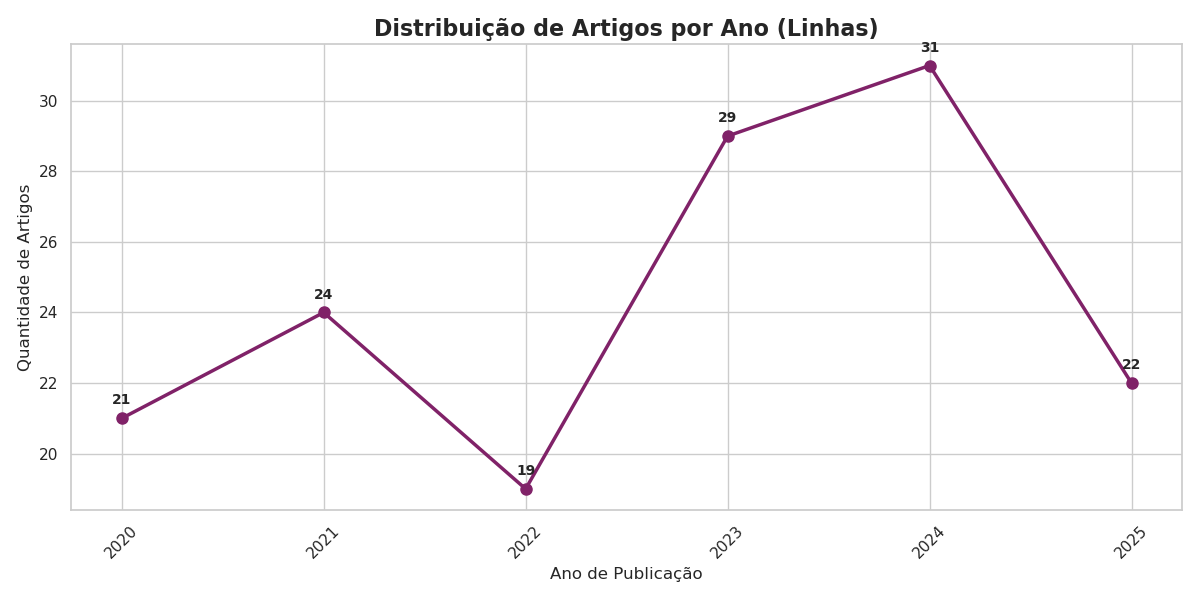
\includegraphics[width=0.65\linewidth]{artigos_por_ano.png}
    \caption{Quantidade de artigos por ano}
    \label{fig:dist_anos}
    {\footnotesize \textit{Fonte: Produção do autor.}}
\end{figure}


Em relação a quantidade de artigos aceitos e rejeitados por base de busca. O ACM  apresentou o maior volume de estudos importados, devido  ao refinamento da busca nos grupos especializados \textit{SIGCSE (Special Interest Group on Computer Science Education)} e \textit{SIGCHI (Special Interest Group on Computer-Human Interaction)}, mas resultou em 2 artigos aceitos. Essa disparidade, justifica-se porque as publicações focam predominantemente com foco em aprendizado em programação.

Além disso, as práticas de gamificação não apresentavam

A figura ~\ref{fig:dist_aceitos_rejeitados} retrata a distribuição de artigos aceitos e rejeitados.
\begin{figure}[H]
    \centering
    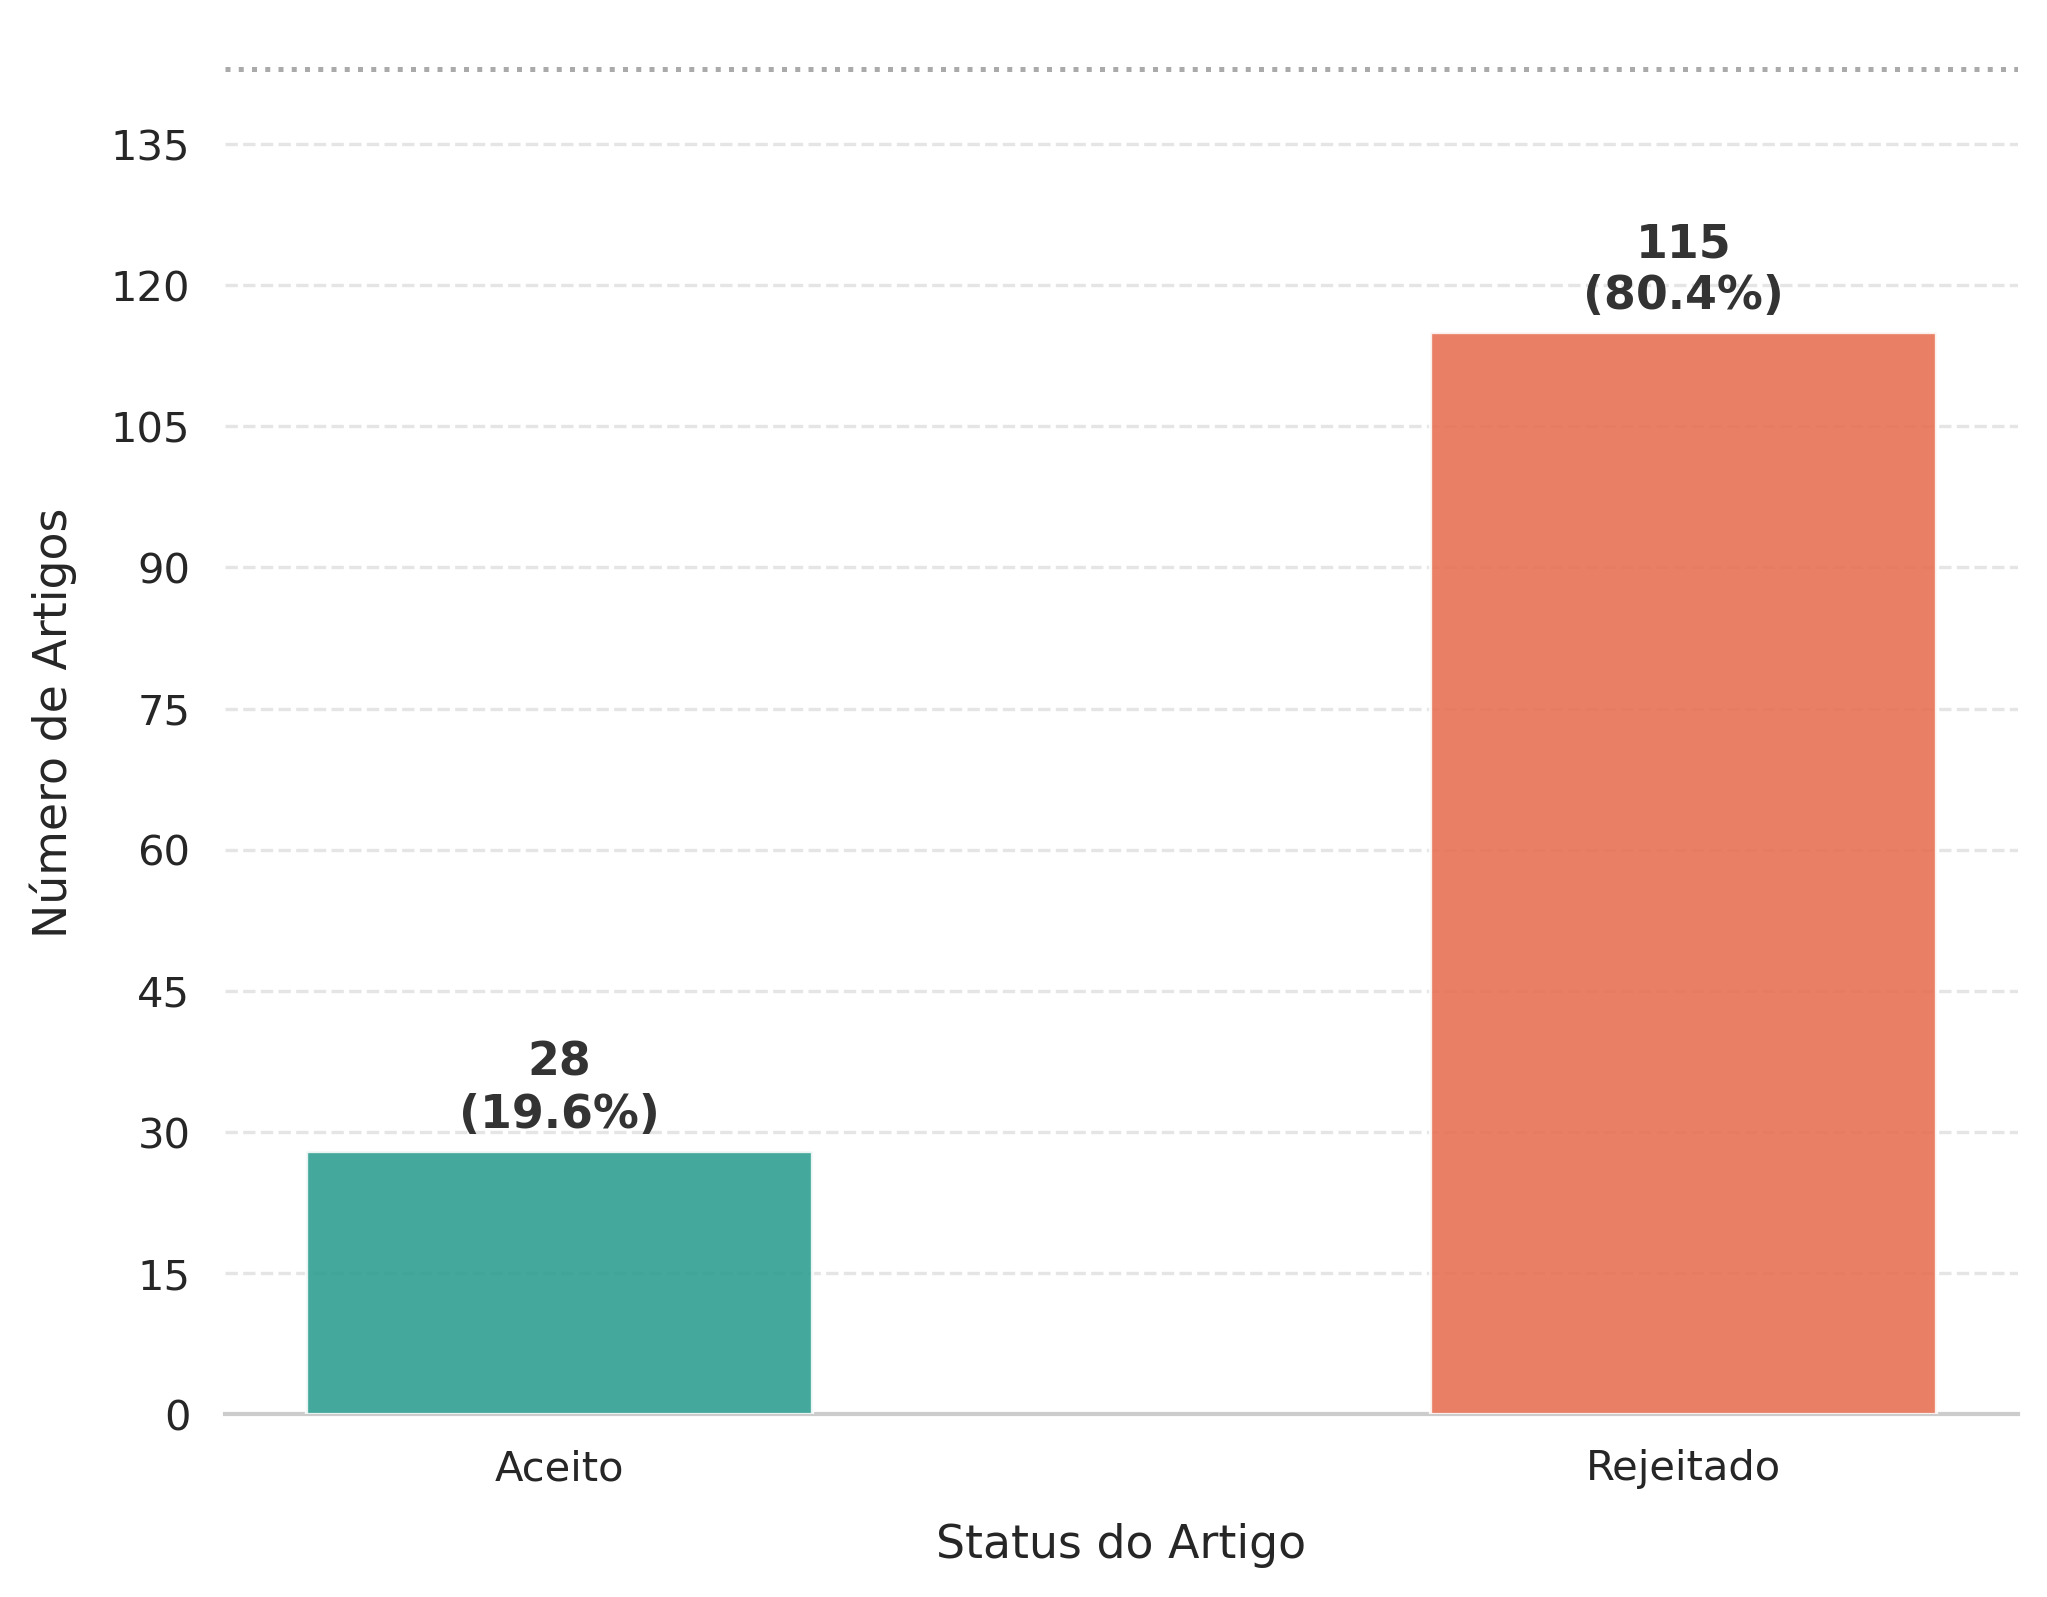
\includegraphics[width=0.65\linewidth]{aceitos_rejeitados.png}
    \caption{Quantidade de artigos aceitos e rejeitados}
    {\footnotesize \textit{Fonte: Produção do autor.}}
    \label{fig:dist_aceitos_rejeitados}
\end{figure}
 alinhamento com o conteúdo matemático de referência desta revisão.

A base \textit{Web Of Science} resultou em 31 artigos importados, 8 aceitos e 22 rejeitados, pois artigos focavam mais em áreas pedagógicas.

Em relação aos rejeitados, os artigos possuem foco em aprendizagem exclusivamente em programação.

A Figura ~\ref{fig:aceitos_rejeitados_por_base} retrata a distribuição de artigos aceitos e rejeitados por base.
\begin{figure}[H]
    \centering
    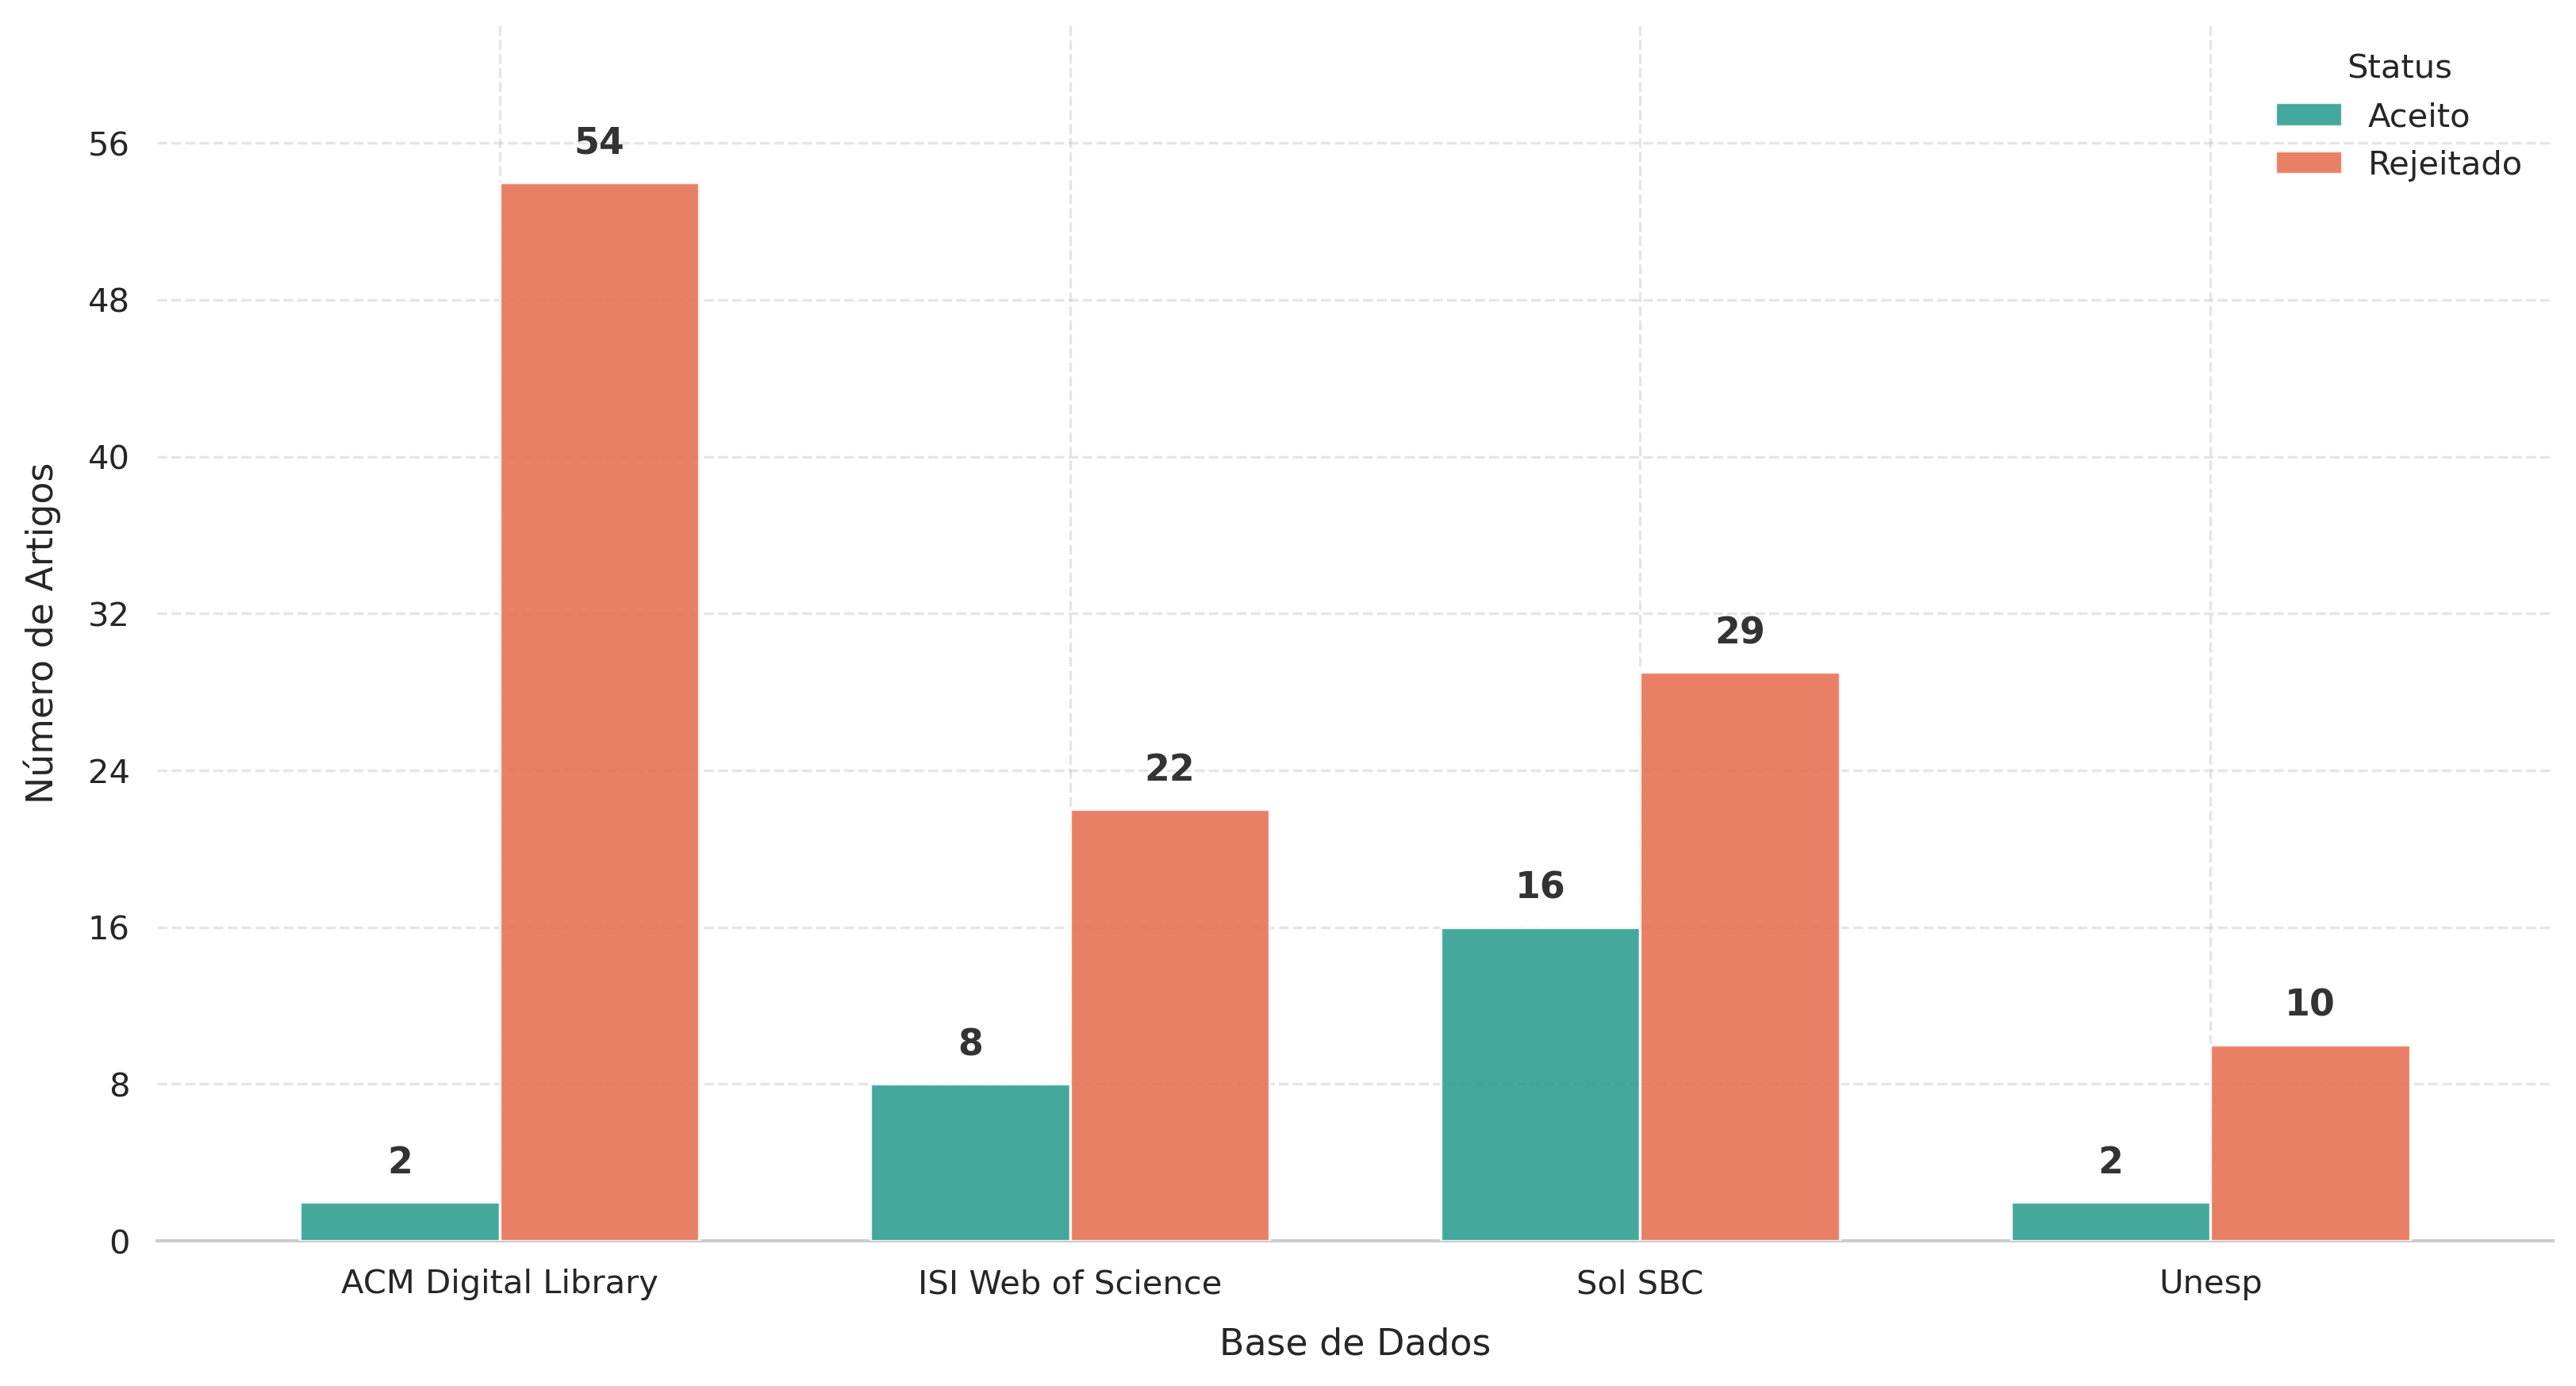
\includegraphics[width=0.65\linewidth]{aceitos_rejeitados_por_base.png}
    \caption{ Distribuição de artigos aceitos e rejeitados por base}
    {\footnotesize \textit{Fonte: Produção do autor.}}
    \label{fig:aceitos_rejeitados_por_base}
\end{figure}

A busca na \textit{SBC-OpenLib} (SOL) resultou na importação de 47 estudos, com 16 artigos aceitos, 29 rejeitados e um não classificado. Isso ocorre, pois a base concentra a produção científica nacional e alinhamento com o contexto do ENEM e BNCC. 

Por fim, a consulta no repositório da UNESP resultou em 12 artigos importados, 2 aceitos. Essa base fornece pesquisas focadas em fundamentações sobre o PC e matemática no ensino brasileiro. 

Logo, as obras das bases \textit{Web Of Science}, SBC e UNESP tendem responder às questões levantadas.

No que tange à distribuição de artigos por critérios. O CI 1 foi mais recorrente, demonstrando que a produção científica concentra no uso de jogos no ensino, já as relações com o PC são menos evidentes.

A Figura ~\ref{fig:artigos_criterio} abaixo retrata a distribuição de artigos pelos critérios de inclusão e exclusão.

\begin{figure}[H]
    \centering
    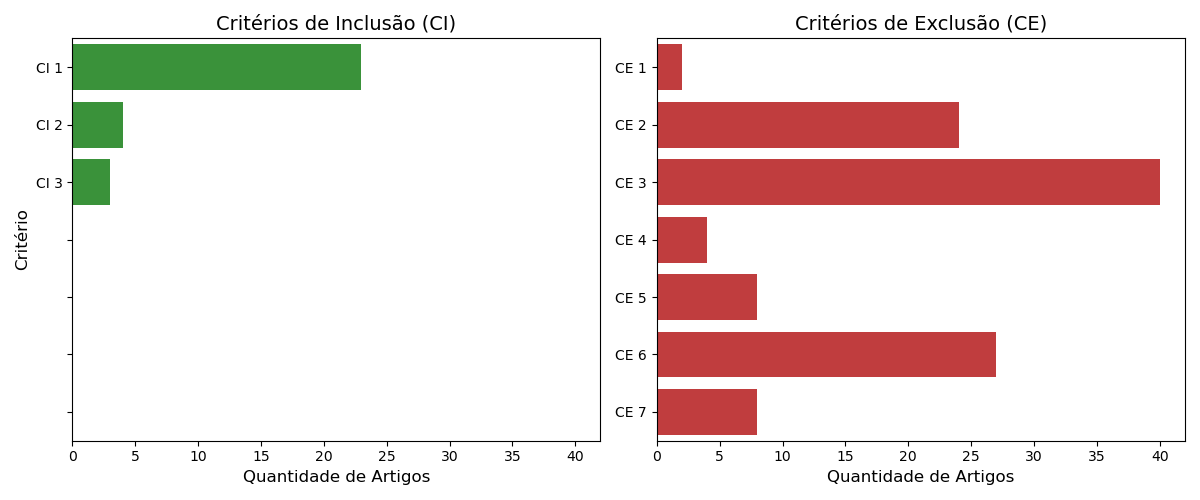
\includegraphics[width=0.65\linewidth]{criterios_juntos_mesma_espessura.png}
    \caption{Quantidade de artigos por critérios.}
    \label{fig:artigos_criterio}
    {\footnotesize \textit{Fonte: Produção do autor.}}
\end{figure}

Quanto aos critérios de exclusão, o mais utilizado foi o (CE 3), que diz respeito a estudos de outras disciplinas ou que não apresentam relação direta com o contexto da revisão. 

O segundo mais aplicado foi o (CE 6), no qual aborda artigos sobre o aprendizado específico em programação.

Em seguida, o CE 2  abrange pesquisas aplicadas exclusivamente ao Ensino Fundamental evidenciando uma significativa produção direcionada aos anos iniciais da educação básica.

Em relação a duplicatas, foi constatado um artigo duplicado (DinoMath: Jogo Sério para o Ensino de Matemática Básica Para Alunos do Ensino Fundamental).

Durante o processo de triagem, identificou-se que o artigo ``Jogo de RPG para o Desenvolvimento de Habilidades do Pensamento Computacional no Ensino Fundamental'' \cite{oliveira2021rpg} é uma extensão do trabalho ``Jogo de RPG para o Desenvolvimento de Habilidades do Pensamento Computacional no Ensino Fundamental: Jogo Digital e Formação de Professores'' \cite{goncalves2022rpg}. Logo, para evitar o viés de duplicação de dados, optou-se pela manutenção do estudo mais recente.

O artigo ``Using the Concept of Game-Based Learning in Education'' \cite{liu2020retracted} foi marcado como não classificado do processo de revisão sistemática após retratação. Foi constatado por terceiros como \textit{paper mill}, uma prática que os artigos são produzidos em massa e vendidos para indivíduos que reivindicam autoria sem terem realizado a pesquisa, conforme documentado pelo portal Retraction Watch \cite{retractionwatch2022investigation} e no histórico de investigações associado aos autores \cite{retractionwatch2022perron}.

\subsection{Análise Qualitativa dos Resultados}

A estruturação de métricas para medir o rigor científico, considerando se os objetivos e motivação estão claramente descritos,validação por pares, se o método da pesquisa está descrito de forma clara e reproduzível. 

Nesse processo, dos 28 artigos passados na triagem, 18 no QA e foram para fase de seleção, para uma nova leitura, buscando filtrar artigos com foco no PC.

Em relação ao público da pesquisa, é avaliado se o estudo envolve estudantes do ensino médio ou ensino fundamental II. Como foi testado os elementos gamificados, se estão descritos, como impacto foi medido e quais os resultados dos testes.

Avalia-se, também como o estudo aborda o conteúdo da disciplina de matemática e se possui relação com os conteúdos cobrados no ENEM.

Por fim, verifica-se os conceitos do PC e a relação com à resolução de problemas.

Outro fator, é a definição de pesos para a criação do \textit{cutoff score} de 8,0. Considerando artigos que respondam mais de 50\% das questões para uma nova leitura. 

A figura  ~\ref{fig:FLUXOGRAMA_PRISMA.png} abaixo retrata o fluxograma implementado nessa revisão.

\begin{figure}[H]
    \centering
    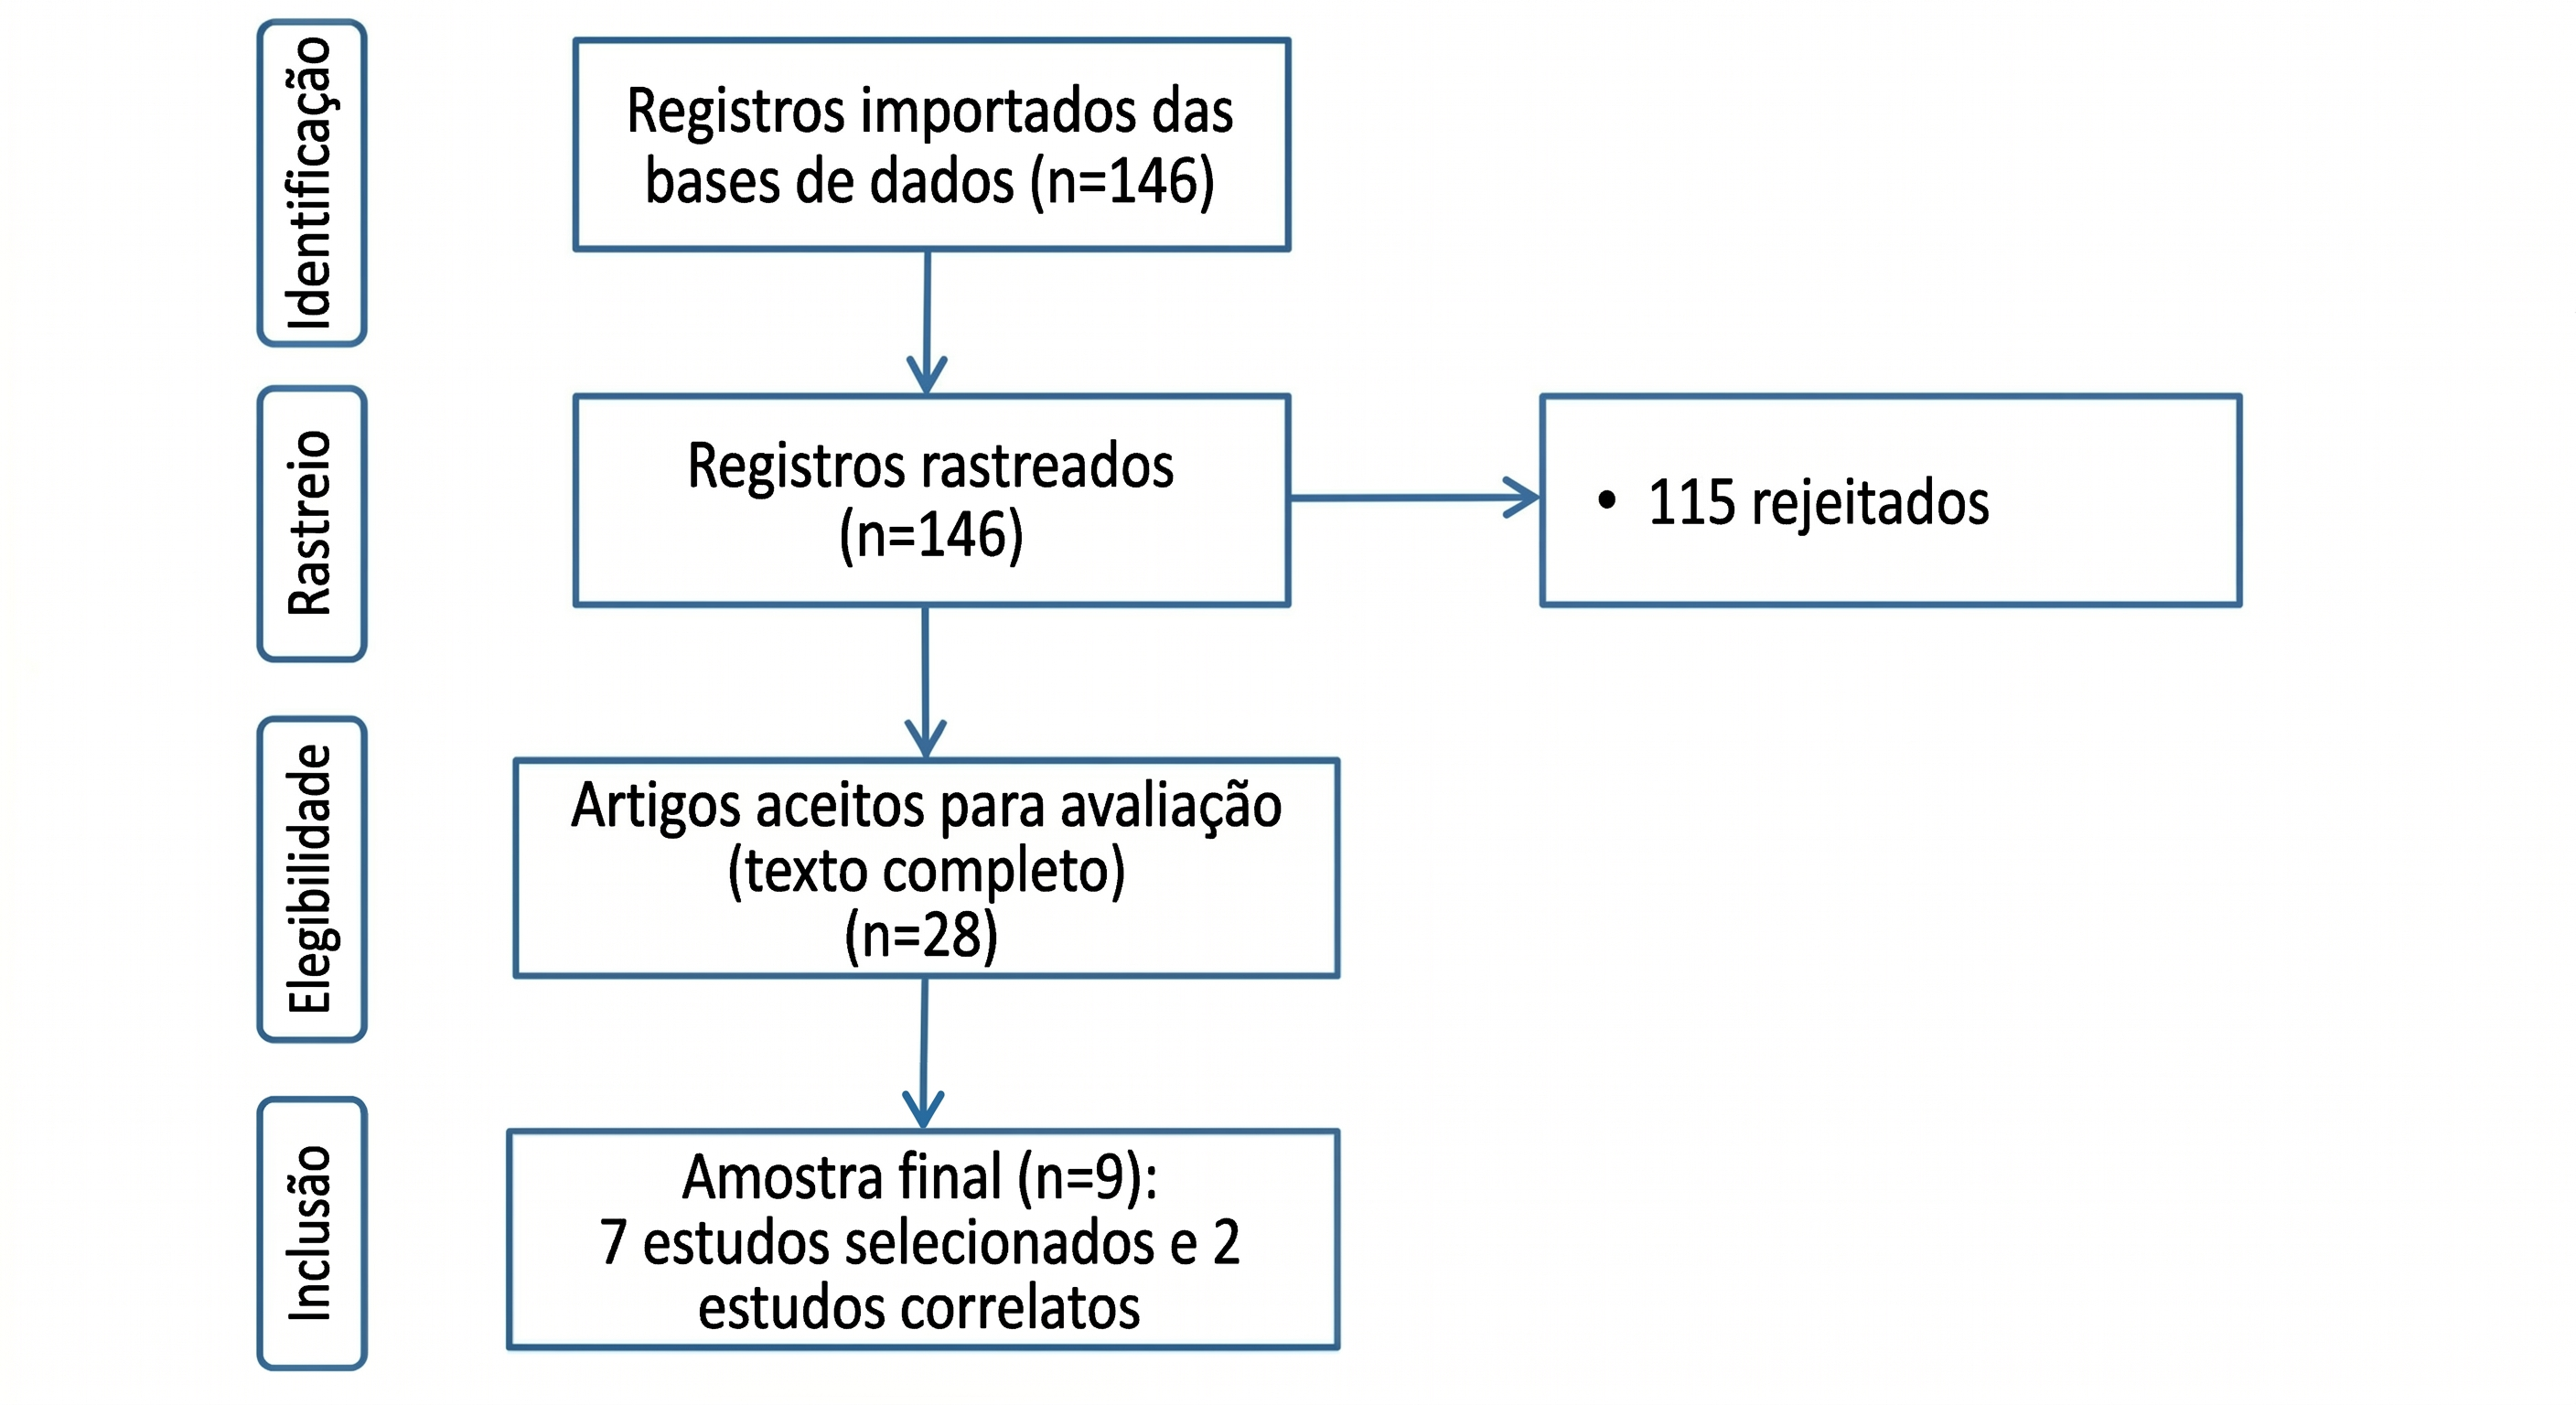
\includegraphics[width=0.65\linewidth]{FLUXOGRAMA_PRISMA.png}
    \caption{Fluxograma}
    \label{fig:FLUXOGRAMA_PRISMA.png}
    {\footnotesize \textit{Fonte: Produção do autor.}}
\end{figure}

\subsubsection{Formulário de Extração e Fase de Seleção}
Nessa fase, foram selecionados 7 artigos que responderam integralmente as questões de pesquisa e 2 estudos correlatos.

\subsubsection{Rabbit Code Um jogo voltado para a aprendizagem de matrizes}
O estudo sobre o Rabbit Code demonstra como a integração entre o pensamento computacional (PC) e sistemas gamificados amplia o engajamento no ensino de matrizes para o nível médio \cite{rolim2023rabbit}. Ao utilizar a gamificação como âncora de conhecimento, o software permite a exploração interativa de conceitos matriciais, superando barreiras de aprendizagem por meio da abstração lúdica de problemas matemáticos \cite{rolim2023rabbit}. A progressão no jogo exige a aplicação obrigatória dos quatro pilares do PC: a decomposição ocorre ao fragmentar o trajeto em blocos de ação; a abstração manifesta-se na análise de linhas e colunas para definir a melhor rota; o reconhecimento de padrões é exercitado ao identificar movimentos para evitar armadilhas; e a criação de algoritmos consolida-se na programação sequencial necessária para atingir os objetivos da fase \cite{rolim2023rabbit}

\subsubsection{Enigmas de Yucatàn: Recurso Educacional Digital para o Ensino de Geometria Espacial}

O artigo sobre Enigmas de Yucatàn  demonstra que o software atrai o aluno por tornar os conceitos de geométria mais intuitivos. No que tange à resolução de problemas matemáticos, o PC contribui ao desenvolver o raciocínio lógico e a abstração, estruturando a mente do estudante para mobilizar o conhecimento e pensar criticamente diante de situações-problema, em vez de depender apenas do uso mecânico de fórmulas \cite{queiros2022enigmas}. 

\subsubsection{Cadê Minha Pizza? Exercitando Matemática e Pensamento Computacional de forma lúdica por meio de grafos}

O artigo demonstra como o PC é desenvolvido com elementos de gamificação e as competências em matemática dos alunos, pois a justificativa para a criação do software baseia-se no potencial dos jogos para os processos de aprendizagem através de motivação e engajamento \cite{honda2023cade}.

O PC contribui ao treinar a estruturação mental do aluno para realizar a modelagem matemática de problemas complexos, pois o jogador deve analisar o mapa, verificar as rotas mais adequadas e enviar o entregador mais adequado para passar de fase, sendo este processo equivalente a percurso em grafos, cálculo do caminho mínimo e alocação de recursos \cite{honda2023cade}.

\subsubsection{Enigma pirata: um jogo para exercitar Matemática e Pensamento Computacional através da Teoria dos Conjuntos}

O estudo atende ao CI 1, pois descreve ativamente o desenvolvimento de um jogo educacional para o ensino de matemática. 

Em primeira análise, a pesquisa preenche o CI 2 ao detalhar de forma extremamente clara como o PC é aplicado na resolução de questões matemáticas. Os autores mapeiam como as ações dos jogadores se alinham aos quatro pilares do PC. 

Por fim, a obra contempla o CI 3, uma vez que o objetivo principal é demonstrar o uso de um jogo digital gamificado de aventura para o desenvolvimento do aprendizado matemático e do PC.

\subsubsection{Atividade de Matemática gamificada com pixel art}
O artigo demonstra que a gamificação por meio de planilhas eletrônicas e pixel art transforma o ambiente educacional ao superar a desmotivação do ensino matemático tradicional \cite{teodosio2023atividade}. Ao atrelar o conteúdo a elementos lúdicos, como recompensas e objetivos, a atividade quebra a resistência dos estudantes e gera um engajamento tão expressivo que até alunos com histórico de baixa participação e rendimento conseguem concluir as tarefas corretamente \cite{teodosio2023atividade}. 

A dinâmica desenvolve o PC, pois o feedback visual imediato da pixel art exige que os alunos apliquem o reconhecimento de padrões para validar seus cálculos, uma vez que a ausência da imagem denuncia o erro \cite{teodosio2023atividade}. Logo, o estudante é induzido a revisar e corrigir seu próprio algoritmo até solucionar a falha.

De acordo com os autores, o aprofundamento dessas metodologias ativas tem o grande potencial de estimular a criatividade, aprimorar o raciocínio lógico e a experiência digital, dentro das perspectivas do Pensamento Computacional \cite{teodosio2023atividade}, competências que fundamentam a capacidade de modelar e interpretar problemas matemáticos complexos.

\subsubsection{O uso das plataformas Scratch e Code.org para o desenvolvimento do Pensamento Computacional na educação básica: relato de experiência alinhado à BNCC}

O estudo atende plenamente ao CI 1, uma vez que relata o uso, o teste e o desenvolvimento prático de jogos digitais especificamente a recriação dos jogos \textit{Pong} e \textit{Geometry Dash} implementando ao ensino de Matemática. 

Em segunda análise, a pesquisa também contempla o CI 2 ao explicar como o PC é utilizado para solucionar problemas de matemática e física na construção dos jogos. Os autores explicam, por exemplo, que os estudantes tiveram que aplicar conceitos do plano cartesiano de maneira prática para solucionar a questão do posicionamento dos personagens no palco da plataforma. \textit{Scratch}, além de detalharem a criação de variáveis matemáticas para simular o efeito da aceleração e da gravidade nos saltos dos avatares \cite{filho2025}. 

Por fim, a obra cumpre integralmente o CI 3, pois o seu objetivo central é validar uma metodologia para o desenvolvimento do Pensamento Computacional utilizando plataformas gamificadas.

\subsubsection{Pensamento computacional e Matemática: uma abordagem com o Scratch}
O estudo atende CI 1, pois descreve  o uso e o desenvolvimento prático de jogos digitais no ensino de Matemática. 

A pesquisa investiga o processo de construção de jogos digitais por meio do \textit{Scratch}, visando o desenvolvimento de habilidades matemáticas orientadas pela (BNCC) \cite{bessa2020}. Além disso, contempla o CI 2, detalhando como o PC é aplicado para resolver problemas matemáticos durante a construção dos jogos. A autora mapeia situações práticas em que os alunos precisaram mobilizar a decomposição (para adequar grandezas de tempo e leitura), criar algoritmos e procedimentos (para gerar movimentos e cálculos de variáveis no plano), e usar a abstração e a análise de dados empíricos, como a proporção e a porcentagem \cite{bessa2020}. 

Por fim, a pesquisa cumpre integralmente o CI 3, uma vez que o seu objetivo geral declarado é investigar o processo de construção de jogos digitais em um ambiente que viabiliza e promove o Pensamento Computacional \cite{bessa2020}.


\subsubsection{Estudos Correlatos}
Embora não integre a amostra de intervenções práticas da revisão sistemática, a dissertação de Silva \cite{silva2020}, entitulada ``Pensamento computacional: uma análise dos documentos oficiais e das questões de Matemática dos vestibulares''. Consolida-se como estudo correlato para estabelecer o referencial teórico ao investigar diretrizes educacionais, como a BNCC, buscando contribuir com a discussão sobre o papel ou não do Pensamento Computacional na Educação Básica\cite{silva2020}.

A autora defende que a sua inserção é fundamental visto que muitas habilidades estão próximas de conceitos matemáticos e o processo de ensino e aprendizagem através do Pensamento Computacional pode contribuir com o desempenho de estudantes\cite{silva2020}. 

Além da fundamentação curricular, a obra destaca-se pelo mapeamento prático dessas competências em questões reais do ENEM e vestibulares paulistas, avaliando potenciais de Abstração e Generalização de Padrões, Algoritmos e Processos, Representação e Automação dos Dados, Decomposição de Problemas e Simulação e Controle de Erros \cite{silva2020}. 

Outra obra correlata é a entitulada: ``Implementation of Gamification in Mathematics m-Learning Application to Creating Student Engagement'' que implementa o \textit{framework Octalysis} e modelo de motivação ARCS (Atenção, Relevância, Confiança e Satisfação)  que consistem em um \textit{design} com ênfase no foco humano para otimizar a motivação, em oposição a um \textit{design} focado apenas em funções de \textit{software} \cite{atin2022}.

\subsection{Planilha Resumo}
A planilha resumo, disponível no \href{https://docs.google.com/spreadsheets/d/1CgtnSKOGnxReo3wmmx0hDnhYqoKaHWd_DOiXrkOBRdQ/edit?usp=sharing}{link}, detalha o processo de seleção dos artigos.
% -----------------------------------------------------------------------
\newpage
\section{Conclusões}

A análise da literatura demonstrou que a utilização de plataformas interativas e de mecânicas de jogos retira o aluno da posição de consumidor passivo, colocando-o como produtor ativo de conhecimento \cite{bessa2020, filho2025}. Tais práticas mostraram-se alinhadas às diretrizes da BNCC que prioriza a incorporação do PC nas aulas de Matemática como uma competência essencial para a modelagem e resolução efetiva de problemas \cite{brasil2017}.

Nesse sentido, a revisão apontou lacunas na literatura, pois parte das práticas gamificadas falham ao não focar no treinamento estruturado do raciocínio exigido, limitando-se a abordagens que apenas fornecem o gabarito final e desconsideram a construção passo a passo do trajeto cognitivo \cite{atin2022implementation}. 

Portanto, as evidências levantadas são o alicerce para elaboração de um anteprojeto de pesquisa que consiste em desenvolver um sistema de aprendizagem gamificado focado no PC, para treinar estudantes na resolução de questões de Matemática do ENEM. A futura ferramenta utilizará o \textit{design} de jogos e elementos de gamificação para  auxiliem na resolução do problema, conectando o PC à proficiência matemática exigida nas avaliações contemporâneas.
\newpage
\bibliographystyle{sbc}
\bibliography{RT1}

\begin{landscape}

\end{landscape}
\end{document}